\documentclass{article}

\usepackage{SDUstyle}

\fancyhf{}
\fancyhead[L]{
    \begin{minipage}[c]{0.2\textwidth}
        \includegraphics[height=11mm]{imgs/logo1.jpg}           %用于设置页眉左侧的图片   Used to set the picture on the left side of the header
    \end{minipage}
}
\fancyhead[C]{实验报告-Experiment report}                        %用于设置页眉中间的文字   Used to set the text in the middle of the header
\fancyfoot[C]{\thepage}
% 设置页眉水平居中
\setlength{\headwidth}{\textwidth}
\fancyhfoffset[L]{\dimexpr0.5\textwidth-0.5\textwidth\relax}

% 设置超链接颜色
\hypersetup{
    colorlinks=true,
    linkcolor=blue, % 超链接的颜色
    urlcolor=red,   % URL 的颜色
    citecolor=green % 引用的颜色
}


\def\singlecover{
\begin{titlepage}                                               %用于单人报告的封面 For single report 
    \centering
    \includegraphics[width=0.65\textwidth]{./imgs/sdured.png}   % 插入你的图片,调整文件名和路径 Insert your picture, adjust the file name and path
    \par\vspace{1.5cm}
    {\Huge \heiti SDU \LaTeX \ Template \par} % 标题 Title
    \vspace{1cm}
    {\Large \heiti 实验报告 Experiment report \par}              % 副标题 Subtitle
    \vspace{5cm}


    % 个人信息  Personal information
    \begin{center}
        {\Large                                                 % 这里的字号也可以用别的方式修改   The font size here can also be modified in other ways
        \makebox[4em][s]{\heiti 姓名}:\underline{\makebox[15em][c]{\heiti 高鹏鸿}}\\
        \makebox[4em][s]{\heiti 学号}:\underline{\makebox[15em][c]{\heiti 000000000000}}\\
        \makebox[4em][s]{\heiti 班级}:\underline{\makebox[15em][c]{\heiti XXX班}}\\
        \makebox[4em][s]{\heiti 学院}:\underline{\makebox[15em][c]{\heiti XXXXXX学院}}\\
        }
    \end{center}

    \vfill
    \today % 日期
\end{titlepage}
}


\def\groupcover{
\begin{titlepage}                                               %用于多人报告的封面 For multiple report
    \centering
    \vspace{1cm}
    \includegraphics[width=0.5\textwidth]{imgs/sdured.png} % 插入你的图片,调整文件名和路径     Insert your picture, adjust the file name and path
    \par\vspace{1cm}
    {\LARGE \heiti 实验报告 Experiment report \par} % 标题     Title
    \vspace{1cm}
    % 组员信息  Group information
    \begin{center}
        \centering
        \textbf{组员1:} 高鹏鸿、 \textbf{组员2:} 1r0ny、 \textbf{组员3:} GPH、 \textbf{组员4:} Irony \\
        \vspace{0.5cm}
        \textbf{组员1学号:} 000000000000 \quad \textbf{班级:} XX一班 \\
        
        \textbf{组员2学号:} 000000000000 \quad \textbf{班级:} XX二班 \\
        
        \textbf{组员3学号:} 000000000000 \quad \textbf{班级:} XX一班 \\
        
        \textbf{组员4学号:} 000000000000 \quad \textbf{班级:} XX二班 \\
        % (其余组员信息类似地添加) (Add the information of other group members in a similar way)
    \end{center}
    
    % 分工情况  Cooperation
    \vspace{2cm}
    \section*{分工情况 Cooperation}
    \addcontentsline{toc}{section}{分工情况 Cooperation}

    \begin{center}
        \begin{tabular}{l}
            组员1 高鹏鸿完成的部分:完成实验报告模板的编写 \\
            组员2 1r0ny完成的部分:完成实验报告模板的编写 \\
            组员3 GPH完成的部分:完成实验报告模板的编写 \\
            组员4 Irony完成的部分:完成实验报告模板的编写 \\
        \end{tabular}
    \end{center}
  
    \vfill
    \today % 日期   Date
\end{titlepage}
}


\begin{document}
\pagenumbering{Roman}
\setcounter{page}{0}

% 切换到单人模式 Switch to single mode
\singlecover

% 切换到多人模式 Switch to multiple mode
\groupcover

\setcounter{page}{1}                                            % 正文页码从 1 开始 The page number of the text starts from 1
\thispagestyle{empty}



\sectionfont{\centering}
\clearpage
\newpage

\setcounter{page}{1}
I
摘要 Abstract
\section*{摘要}
\addcontentsline{toc}{section}{摘要 Abstract}                            %用来目录中添加相应的条目   Add the corresponding entry in the table of contents

这个实验报告模板介绍了如何使用 \LaTeX 来编写实验报告,包括了一些基本的使用方法,例如插入图片、插入代码、插入表格、插入公式、插入参考文献、插入超链接、插入脚注、绘制图像等。以及一些这个模板专有的一些使用方法,例如封面的设置、页眉页脚的设置等。如果喜欢的而话可以去我的github界面点个star:\href{https://github.com/AlmostGPH/SDU-Latex-Template-for-Document}{https://github.com/AlmostGPH/SDU-Latex-Template-for-Document}

\section*{Abstract}

This experiment report template introduces how to use \LaTeX to write experiment reports, including some basic usage methods, such as inserting pictures, inserting code, inserting tables, inserting formulas, inserting references, inserting hyperlinks, inserting footnotes, drawing images, etc. And some specific usage methods of this template, such as setting the cover, setting the header and footer, etc. If you like it, you can go to my github interface and give it a star: \href{https://github.com/AlmostGPH/SDU-Latex-Template-for-Document}{https://github.com/AlmostGPH/SDU-Latex-Template-for-Document}

\clearpage

\addcontentsline{toc}{section}{目录 Table of Contents}
II
目录 Table of Contents
\thispagestyle{empty}
\hypersetup{linkcolor=black}
\tableofcontents
\hypersetup{linkcolor=blue}
\newpage


\setcounter{page}{1}
\pagenumbering{arabic}

\section{SDU \LaTeX 模板介绍 Introduction}

这个模板通过结合一些现有的模板和一些文章由 \href{https://github.com/AlmostGPH}{高鹏鸿} 实现,在GNU通用公共许可证下发布。在编译时请使用 {\bf XeLaTex}

\vspace{0.5cm}

This template is implemented by combining some existing templates and some articles by \href{https://github.com/AlmostGPH}{Penghong Gao}. It is released under the GNU General Public License. Use {\bf XeLaTex} when compiling.

\vspace{0.5cm}


如果你在使用此模板时遇到任何问题,请联系 \href{2861126078@qq.com}{2861126078@qq.com} 下面是一些简单的介绍
\vspace{0.5cm}

If you encounter any problems when using this template, please contact \href{2861126078@qq.com}{2861126078@qq.com} Here are some simple introductions.

\subsection{基本使用 Basic Usage}

\subsubsection{段落以及空行 Paragraph and Blank Line}

直接在代码中输入文字就是新成一段,更换段落之间需要空一行。

If you want to start a new paragraph, just type the text directly in the code, and you need to leave a blank line between paragraphs.

\vspace{0.5cm}

想要空一行可以使用 \verb|vspace{0.5cm}| 来实现

If you want to leave a blank line, you can use \verb|vspace{0.5cm}| to achieve it.

\begin{lstlisting}[
    style       =   TeX,
    caption     =   {\bf 段落和空行 Paragraph and Blank Line},
    label       =   {para}
]
直接在代码中输入文字就是新成一段,更换段落之间需要空一行。

If you want to start a new paragraph, just type the text directly in the code, and you need to leave a blank line between paragraphs.

\vspace{0.5cm}

想要空一行可以使用 \verb|vspace{0.5cm}| 来实现

If you want to leave a blank line, you can use \verb|vspace{0.5cm}| to achieve it.

\end{lstlisting}

\subsubsection{itemize环境 Itemize Environment}

\begin{itemize}
    \item 第一项 First item
    \subitem 第一项子项 First subitem   
    \item 第二项 Second item    
    \item 第三项 Third item
\end{itemize}

\clearpage

\begin{lstlisting}[
    style       =   TeX,
    caption     =   {\bf 使用itemize环境},
    label       =   {item}
]
\begin{itemize}
    \item 第一项 First item
    \subitem 第一项子项 First subitem   
    \item 第二项 Second item    
    \item 第三项 Third item
\end{itemize}
\end{lstlisting}

\subsubsection{行间代码 Inline Code}

行间代码可以使用 \verb|\verb| 命令来实现,例如 \verb|print("Hello, World!")|。

Inline code can be implemented using the \verb|\verb| command, for example, \verb|print("Hello, World!")|.

\begin{lstlisting}[
    style       =   TeX,
    caption     =   {\bf 行间代码 Inline Code},
    label       =   {inline}
]
行间代码可以使用 \verb|\verb| 命令来实现,例如 \verb|print("Hello, World!")|。

Inline code can be implemented using the \verb|\verb| command, for example, \verb|print("Hello, World!")|.

\end{lstlisting}

\subsubsection{使用分栏 Using Columns}

\begin{multicols}{2} % 指定两列
    这是左栏 This is the left column

    hello world

    \columnbreak % 在这里可以手动换列

    这是右栏 This is the right column

    你好
\end{multicols}

\begin{lstlisting}[
    style       =   TeX,
    caption     =   {\bf 使用分栏 Using Columns},
    label       =   {column}
]
\begin{multicols}{2} % 指定两列
    这是左栏 This is the left column

    hello world

    \columnbreak % 在这里可以手动换列

    这是右栏 This is the right column

    你好
\end{multicols}
\end{lstlisting}

更多使用方式可以查看 \href{https://www.overleaf.com/learn/latex/Multiple_columns}{这里}。

More usage can be found \href{https://www.overleaf.com/learn/latex/Multiple_columns}{here}.


\subsection{插入图片 Insert Picture}

插入图片可以使用 \verb|\includegraphics| 命令,如图\ref{fig:1}所示。

Inserting pictures can be done using the \verb|\includegraphics| command, as shown in Figure \ref{fig:1}.

\clearpage

\begin{figure}[htbp]
    \begin{center}
        \includegraphics[width=0.8\textwidth]{imgs/logo1.jpg}
        \caption{SDU Logo}
        \label{fig:1}
    \end{center}
\end{figure}

\begin{lstlisting}[
    style       =   TeX,
    caption     =   {\bf 插入图片 Insert Picture},
    label       =   {imgs}
]
\begin{figure}[htbp] % htbp表示图片位置,h表示here,t表示top,b表示bottom,p表示page
    \begin{center}
        \includegraphics[width=0.8\textwidth]{imgs/logo1.jpg}% width调整图片大小 width adjusts the size of the picture
        \caption{SDU Logo}
        \label{fig:1}
    \end{center}
\end{figure}
\end{lstlisting}


\subsection{插入代码 Insert Code}

这个模板中插入模板的方式基于\href{https://zhuanlan.zhihu.com/p/65441079}{这篇文章}进行迭代修改

The way to insert code in this template is based on \href{https://zhuanlan.zhihu.com/p/65441079}{this article} for iterative modification.


\subsubsection{代码写在内部文件 Code in Internal File}

\begin{lstlisting}[
    style       =   TeX,
    caption     =   {\bf 代码写在内部文件 Code in Internal File},
    label       =   {code}
]
\begin{lstlisting}[
    style       =   TeX,
    caption     =   {\bf 示例标题 Title},
    label       =   {title}
]
codes
codes
...
{用于闭合的代码 Closing code}
\end{lstlisting}  %代码块需要用\end{lstlisting}闭合,但是这里如果写进去的话会导致编译器无法分辨,所以这里没有加 To close the code block, you need to use \end{lstlisting}, but if you write it in here, the compiler will not be able to distinguish, so it is not added here.

代码块需要用 \verb|\end{lstlisting}| 闭合,但是这里如果写进去的话会导致编译器无法分辨,所以这里没有加。在使用其他代码或者使用外部文件引用时不会出现这样的问题,所以推荐使用外部文件引用。

The code block needs to be closed with \verb|\end{lstlisting}|, but if you write it in here, the compiler will not be able to distinguish, so it is not added here. There will be no such problem when using other code or using external file references, so it is recommended to use external file references.


\vspace{0.5cm}

也能这么写:

It can also be written like this:

\begin{lstlisting}[style = TeX, caption = {\bf 代码写在内部文件 Code in Internal File}, label = {code}]
\begin{lstlisting}[style = TeX, caption = {\bf 示例标题 Title}, label = {title}]
codes
codes
...

{用于闭合的代码 Closing code}
\end{lstlisting}


\vspace{0.5cm}

Python代码示例:

Python code example:

\begin{lstlisting}[
    style       =   Python,
    caption     =   {\bf Python示例 Python Example},
    label       =   {py}
]
def extended_gcd(a, b):
    if b == 0:
        return (a, 1, 0)
    else:
        d, x, y = extended_gcd(b, a % b)
        return (d, y, x - (a // b) * y)


def mod_inverse(a, m):
    d, x, y = extended_gcd(a, m)
    if d != 1:
        raise ValueError("Modular inverse does not exist")
    else:
        return x % m
\end{lstlisting}



\subsubsection{代码写在外部文件 Code in External File}

\begin{lstlisting}[
    style       =   TeX,
    caption     =   {\bf 代码写在外部文件 Code in External File},
    label       =   {out}
]
\lstinputlisting[
    style       =   TeX,
    caption     =   {\bf 示例标题 Title},
    label       =   {test}
]{codes/temp.tex} %代码文件的相对路径 The relative path of the code file
\end{lstlisting} 

\lstinputlisting[
    style       =   TeX,
    caption     =   {\bf TeX示例 TeX Example},
    label       =   {texOut}
]{codes/temp.tex} %代码文件的相对路径 The relative path of the code file


\vspace{0.5cm}

Python代码示例:

Python code example:

\lstinputlisting[
    style       =   Python,
    caption     =   {\bf Python示例 Python Example},
    label       =   {PythonOut}
]{codes/temp.py}



\subsection{插入表格 Insert Table}

\begin{multicols}{2} % 指定两列

    \centering
    \captionof{table}{表格示例1 Table Example 1}        % 使用captionof命令来实现表格标题 Use the captionof command to achieve the table title
    \label{tab:tab1}
    \begin{tabular}{|c|c|c|}                            % “|”表示竖线,“c”表示居中,“l”表示左对齐,“r”表示右对齐,“||”表示双竖线    
        \hline                                          % 用\hline表示横线 Use \hline to indicate the horizontal line
        A & B & C \\
        \hline
        1 & 2 & 3 \\
        \hline
        4 & 5 & 6 \\
        \hline
        7 & 8 & 9 \\
        \hline
    \end{tabular}
    
    \columnbreak % 在这里可以手动换行
    
    \centering
    \captionof{table}{表格示例2 Table Example 2}        % 示例 2 Example 2 
    \label{tab:tab2}
    \begin{tabular}{r||l c|}
        \hline
        AA & BB & C \\
        \hline
        1 & 2 & 3 \\
        4 & 5 & 6 \\
        \hline
        \hline
        7 & 8 & 9 \\
    \end{tabular}
    
\end{multicols}

\begin{lstlisting}[
    style       =   TeX,
    caption     =   {\bf 插入表格 Insert Table},
    label       =   {table}
]
\begin{multicols}{2} % 指定两列

    \centering
    \captionof{table}{表格示例1 Table Example 1}        % 使用captionof命令来实现表格标题 Use the captionof command to achieve the table title
    \label{tab:tab1}
    \begin{tabular}{|c|c|c|}                            % “|”表示竖线,“c”表示居中,“l”表示左对齐,“r”表示右对齐,“||”表示双竖线    
        \hline                                          % 用\hline表示横线 Use \hline to indicate the horizontal line
        A & B & C \\
        \hline
        1 & 2 & 3 \\
        \hline
        4 & 5 & 6 \\
        \hline
        7 & 8 & 9 \\
        \hline
    \end{tabular}
    
    \columnbreak % 在这里可以手动换行
    
    \centering
    \captionof{table}{表格示例2 Table Example 2}        % 示例 2 Example 2 
    \label{tab:tab2}
    \begin{tabular}{r||l c|}
        \hline
        AA & BB & CC \\
        \hline
        1 & 2 & 3 \\
        4 & 5 & 6 \\
        \hline
        \hline
        7 & 8 & 9 \\
    \end{tabular}
    
\end{multicols}
\end{lstlisting}

\subsection{插入公式 Insert Formula}

如果不想学习 \LaTeX 的公式语法,可以使用 \href{https://www.codecogs.com/latex/eqneditor.php}{CodeCogs} 来生成公式的代码。

If you don't want to learn the formula syntax of \LaTeX, you can use \href{https://www.codecogs.com/latex/eqneditor.php}{CodeCogs} to generate the code of the formula.

\subsubsection{行内公式 Inline Formula}

行内公式可以使用 \verb|$...$| 或者 \verb|\(...\)| 来实现,例如 $a^2 + b^2 = c^2$ 或者 \((a+b)^2 = a^2 + 2ab + b^2\)。

Inline formulas can be implemented using \verb|$...$| or \verb|\(...\)|, for example, $a^2 + b^2 = c^2$ or \((a+b)^2 = a^2 + 2ab + b^2\).

\begin{lstlisting}[
    style       =   TeX,
    caption     =   {\bf 行内公式 Inline Formula},
    label       =   {inlinef}
]
行内公式可以使用 \verb|$...$| 或者 \verb|\(...\)| 来实现,例如 $a^2 + b^2 = c^2$ 或者 \((a+b)^2 = a^2 + 2ab + b^2\)。

Inline formulas can be implemented using \verb|$...$| or \verb|\(...\)|, for example, $a^2 + b^2 = c^2$ or \((a+b)^2 = a^2 + 2ab + b^2\).
\end{lstlisting}

\subsubsection{行间公式 Display Formula}

行间公式可以使用 \verb|\[...\]| 或者 \verb|\begin{equation}...\end{equation}| 来实现,例如:

Display formulas can be implemented using \verb|\[...\]| or \verb|\begin{equation}...\end{equation}|, for example:


\[
    \int_{0}^{1} x^2 \, dx = \frac{1}{3}
\]


\begin{equation}
    \int_{0}^{1} x^2 \, dx = \frac{1}{3}
\end{equation}


\begin{lstlisting}[
    style       =   TeX,
    caption     =   {\bf 行间公式 Display Formula},
    label       =   {displayf}
]
\[
    \int_{0}^{1} x^2 \, dx = \frac{1}{3}
\]

\begin{equation}
    \int_{0}^{1} x^2 \, dx = \frac{1}{3}
\end{equation}

\end{lstlisting}



\subsection{插入参考文献 Insert Reference}

\subsubsection{内部参考文献 Internal Reference}

内部参考文献可以使用 \verb|\label| 和 \verb|\ref| 来实现,首先使用 \verb|\label| 定义一个标签,然后使用 \verb|\ref| 来引用这个东西,例如: “表格的用法如表 \ref{tab:tab2} 所示”。然后点击“表 \ref{tab:tab2}”就能跳转到相应位置

Internal references can be implemented using \verb|\label| and \verb|\ref|. First, use \verb|\label| to define a label, and then use \verb|\ref| to reference it, for example: “The usage of tables is shown in Table \ref{tab:tab2}”. Then click on “Table \ref{tab:tab2}” to jump to the corresponding position.

\begin{lstlisting}[
    style       =   TeX,
    caption     =   {\bf 内部参考文献 Internal Reference},
    label       =   {ref}
]
\captionof{table}{表格示例2 Table Example 2}
\label{tab:tab2} % 定义一个标签 Define a label
\begin{tabular}{r||l c|}
    \hline
    AA & BB & C \\
    \hline
    1 & 2 & 3 \\
    4 & 5 & 6 \\
    \hline
    \hline
    7 & 8 & 9 \\
\end{tabular}
...
...
...
内部参考文献可以使用 \verb|\label| 和 \verb|\ref| 来实现,首先使用 \verb|\label| 定义一个标签,然后使用 \verb|\ref| 来引用这个东西,例如: “表格的用法如表 \ref{tab:tab2} 所示”。然后点击“表 \ref{tab:tab2}”就能跳转到相应位置

Internal references can be implemented using \verb|\label| and \verb|\ref|. First, use \verb|\label| to define a label, and then use \verb|\ref| to reference it, for example: “The usage of tables is shown in Table \ref{tab:tab2}”. Then click on “Table \ref{tab:tab2}” to jump to the corresponding position.
\end{lstlisting}

\subsubsection{外部参考文献 External Reference}

外部参考文献可以使用 \verb|\bibitem| 和 \verb|\cite| 来实现,首先使用 \verb|\bibitem| 定义一个参考文献,然后使用 \verb|\cite| 来引用这个东西,例如: “这是一个外部参考文献 \cite{1}”。

External references can be implemented using \verb|\bibitem| and \verb|\cite|. First, use \verb|\bibitem| to define a reference, and then use \verb|\cite| to reference it, for example: “This is an external reference \cite{1}”.

\clearpage

\begin{lstlisting}[
    style       =   TeX,
    caption     =   {\bf 外部参考文献 External Reference},
    label       =   {cite}
]
外部参考文献可以使用 \verb|\bibitem| 和 \verb|\cite| 来实现,首先使用 \verb|\bibitem| 定义一个参考文献,然后使用 \verb|\cite| 来引用这个东西,例如: “这是一个外部参考文献 \cite{1}”。

External references can be implemented using \verb|\bibitem| and \verb|\cite|. First, use \verb|\bibitem| to define a reference, and then use \verb|\cite| to reference it, for example: “This is an external reference \cite{1}”.
...
...
...
\begin{thebibliography}{9}
    \bibitem{1} Gao P H. SDU \LaTeX \ Template[J]. 2024
\end{thebibliography}


\end{lstlisting}

\subsection{插入超链接 Insert Hyperlink}

超链接可以使用 \verb|\href{链接}{文档中显示文本}| 来实现,例如: \\这是我的博客:\href{https://almostgph.github.io/}{https://almostgph.github.io/}。

Hyperlinks can be implemented using \verb|\href{link}{text in document}|, for example: \\This is my blog: \href{https://almostgph.github.io/}{https://almostgph.github.io/}.

\begin{lstlisting}[
    style       =   TeX,
    caption     =   {\bf 插入超链接 Insert Hyperlink},
    label       =   {hyper}
]
超链接可以使用 \verb|\href{链接}{文档中显示文本}| 来实现,例如: 这是我的博客:\href{https://almostgph.github.io/}{https://almostgph.github.io/}。

Hyperlinks can be implemented using \verb|\href{link}{text in document}|, for example: This is my blog: \href{https://almostgph.github.io/}{https://almostgph.github.io/}.
\end{lstlisting}

\subsection{插入脚注 Insert Footnote}

脚注可以使用 \verb|\footnote{脚注内容}| 来实现,例如:这是一个脚注\footnote{这是一个脚注}。

Footnotes can be implemented using \verb|\footnote{footnote content}|, for example: This is a footnote\footnote{This is a footnote}.

\clearpage

\begin{lstlisting}[
    style       =   TeX,
    caption     =   {\bf 插入脚注 Insert Footnote},
    label       =   {foot}
]
脚注可以使用 \verb|\footnote{脚注内容}| 来实现,例如:这是一个脚注\footnote{这是一个脚注}。

Footnotes can be implemented using \verb|\footnote{footnote content}|, for example: This is a footnote\footnote{This is a footnote}.
\end{lstlisting}

\subsection{绘制图像 Draw Image}

使用tikz包可以绘制各种图像,例如流程图、树图等。这里只是简单的举例使用,如果想要详细和深度的了解,可以查看 \href{https://cn.overleaf.com/learn/latex/TikZ_package}{https://cn.overleaf.com/learn/latex/TikZ\_package}。

The tikz package can be used to draw various images, such as flowcharts, tree diagrams, etc. Here is just a simple example. If you want to know more details, you can check\\ \href{https://cn.overleaf.com/learn/latex/TikZ_package}{https://cn.overleaf.com/learn/latex/TikZ\_package}.

\subsubsection{绘制流程图 Draw Flowchart}


\begin{figure}[htbp]
    \centering
    \begin{tikzpicture}[node distance=1.5cm]
        \usetikzlibrary{shapes,arrows}

        \tikzstyle{startstop} = [rectangle, rounded corners, minimum width=3cm, minimum height=1cm, text centered, draw=black, fill=red!30]
        \tikzstyle{io} = [trapezium, trapezium left angle=70, trapezium right angle=110, minimum width=3cm, minimum height=1cm, text centered, draw=black, fill=blue!30]
        \tikzstyle{process} = [rectangle, minimum width=3cm, minimum height=1cm, text centered, draw=black, fill=orange!30]
        \tikzstyle{decision} = [diamond, minimum width=3cm, minimum height=1cm, text centered, draw=black, fill=green!30]
        \tikzstyle{arrow} = [thick,->,>=stealth]

        \node (start) [startstop] {Start};
        \node (in1) [io, below of=start] {Input};
        \node (pro1) [process, below of=in1] {Process 1};
        \node (dec1) [decision, below of=pro1, yshift=-0.5cm] {Decision 1};
        \node (pro2a) [process, below of=dec1, yshift=-0.5cm] {Process 2a};
        \node (pro2b) [process, right of=dec1, xshift=2cm] {Process 2b};
        \node (out1) [io, below of=pro2a] {Output};
        \node (stop) [startstop, below of=out1] {Stop};
        
        \draw [arrow] (start) -- (in1);
        \draw [arrow] (in1) -- (pro1);
        \draw [arrow] (pro1) -- (dec1);
        \draw [arrow] (dec1) -- node[anchor=east] {yes} (pro2a);
        \draw [arrow] (dec1) -- node[anchor=south] {no} (pro2b);
        \draw [arrow] (pro2b) |- (pro1);
        \draw [arrow] (pro2a) -- (out1);
        \draw [arrow] (out1) -- (stop);
    \end{tikzpicture}
    \caption{流程图 Flowchart}
    \label{fig:flowchart}
\end{figure}

\clearpage


\begin{lstlisting}[
    style       =   TeX,
    caption     =   {\bf 绘制流程图 Draw Flowchart},
    label       =   {flowchart}
]
\begin{figure}[htbp]
    \centering
    \begin{tikzpicture}[node distance=1.5cm]
        \usetikzlibrary{shapes,arrows}

        \tikzstyle{startstop} = [rectangle, rounded corners, minimum width=3cm, minimum height=1cm, text centered, draw=black, fill=red!30]
        \tikzstyle{io} = [trapezium, trapezium left angle=70, trapezium right angle=110, minimum width=3cm, minimum height=1cm, text centered, draw=black, fill=blue!30]
        \tikzstyle{process} = [rectangle, minimum width=3cm, minimum height=1cm, text centered, draw=black, fill=orange!30]
        \tikzstyle{decision} = [diamond, minimum width=3cm, minimum height=1cm, text centered, draw=black, fill=green!30]
        \tikzstyle{arrow} = [thick,->,>=stealth]

        \node (start) [startstop] {Start};
        \node (in1) [io, below of=start] {Input};
        \node (pro1) [process, below of=in1] {Process 1};
        \node (dec1) [decision, below of=pro1, yshift=-0.5cm] {Decision 1};
        \node (pro2a) [process, below of=dec1, yshift=-0.5cm] {Process 2a};
        \node (pro2b) [process, right of=dec1, xshift=2cm] {Process 2b};
        \node (out1) [io, below of=pro2a] {Output};
        \node (stop) [startstop, below of=out1] {Stop};
        
        \draw [arrow] (start) -- (in1);
        \draw [arrow] (in1) -- (pro1);
        \draw [arrow] (pro1) -- (dec1);
        \draw [arrow] (dec1) -- node[anchor=east] {yes} (pro2a);
        \draw [arrow] (dec1) -- node[anchor=south] {no} (pro2b);
        \draw [arrow] (pro2b) |- (pro1);
        \draw [arrow] (pro2a) -- (out1);
        \draw [arrow] (out1) -- (stop);
    \end{tikzpicture}
    \caption{流程图 Flowchart}
    \label{fig:flowchart}
\end{figure}
\end{lstlisting}

\clearpage

\subsubsection{绘制树图 Draw Tree Diagram}

\begin{figure}[htbp]
    \centering
    \begin{tikzpicture}[sibling distance=10em,
        every node/.style = {shape=rectangle, rounded corners,
            draw, align=center,
            top color=white, bottom color=blue!20}]]
        \node {Root}
        child { node {Child 1} 
            child { node {Grandchild 1} }
            child { node {Grandchild 2} }
        }
        child { node {Child 2} 
            child { node {Grandchild 3} }
            child { node {Grandchild 4} }
        };
    \end{tikzpicture}
    \caption{树图 Tree Diagram}
    \label{fig:tree}
\end{figure}

\begin{lstlisting}[
    style       =   TeX,
    caption     =   {\bf 绘制树图 Draw Tree Diagram},
    label       =   {tree}
]

\begin{figure}[htbp]
    \centering
    \begin{tikzpicture}[sibling distance=10em,
        every node/.style = {shape=rectangle, rounded corners,
            draw, align=center,
            top color=white, bottom color=blue!20}]]
        \node {Root}
        child { node {Child 1} 
            child { node {Grandchild 1} }
            child { node {Grandchild 2} }
        }
        child { node {Child 2} 
            child { node {Grandchild 3} }
            child { node {Grandchild 4} }
        };
    \end{tikzpicture}
    \caption{树图 Tree Diagram}
    \label{fig:tree}
\end{figure}
\end{lstlisting}




\subsubsection{绘制拓扑图 Draw Topology Diagram}

\begin{figure}[htbp]
    \centering
    \begin{tikzpicture}
        \usetikzlibrary{positioning}
        \node (A) {A};
        \node (B) [right=of A] {B};
        \node (C) [below=of A] {C};
        \node (D) [below=of B] {D};
        \draw (A) -- (B);
        \draw (A) -- (C);
        \draw (B) -- (D);
        \draw (C) -- (D);
    \end{tikzpicture}
    \caption{拓扑图 Topology Diagram}
    \label{fig:topology}
\end{figure}

\clearpage

\begin{lstlisting}[
    style       =   TeX,
    caption     =   {\bf 绘制拓扑图 Draw Topology Diagram},
    label       =   {topology}
]
\begin{figure}[htbp]
    \centering
    \begin{tikzpicture}
        \usetikzlibrary{positioning}
        \node (A) {A};
        \node (B) [right=of A] {B};
        \node (C) [below=of A] {C};
        \node (D) [below=of B] {D};
        \draw (A) -- (B);
        \draw (A) -- (C);
        \draw (B) -- (D);
        \draw (C) -- (D);
    \end{tikzpicture}
    \caption{拓扑图 Topology Diagram}
    \label{fig:topology}
\end{figure}
\end{lstlisting}


\subsubsection{绘制时序图 Draw Timing Diagram}

\begin{figure}[htbp]
    \centering
    \begin{tikzpicture}
        \draw (0,0) -- (0,1) -- (1,1) -- (1,0) -- (2,0) -- (2,1) -- (3,1) -- (3,0) -- (4,0);
    \end{tikzpicture}
    \caption{时序图 Timing Diagram}
    \label{fig:timing}
\end{figure}

\begin{lstlisting}[
    style       =   TeX,
    caption     =   {\bf 绘制时序图 Draw Timing Diagram},
    label       =   {timing}
]
\begin{figure}[htbp]
    \centering
    \begin{tikzpicture}
        \draw (0,0) -- (0,1) -- (1,1) -- (1,0) -- (2,0) -- (2,1) -- (3,1) -- (3,0) -- (4,0);
    \end{tikzpicture}
    \caption{时序图 Timing Diagram}
    \label{fig:timing}
\end{figure}
\end{lstlisting}

\clearpage

\subsubsection{绘制其他图 Draw Other Diagram}

\begin{figure}[htbp]
    \centering
    \begin{tikzpicture}
        \draw (0,0) circle [radius=1];
    \end{tikzpicture}
    \caption{其他图 Other Diagram}
    \label{fig:other}
\end{figure}

\begin{lstlisting}[
    style       =   TeX,
    caption     =   {\bf 绘制其他图 Draw Other Diagram},
    label       =   {other}
]
\begin{figure}[htbp]
    \centering
    \begin{tikzpicture}
        \draw (0,0) circle [radius=1];
    \end{tikzpicture}
    \caption{其他图 Other Diagram}
    \label{fig:other}
\end{figure}
\end{lstlisting}

\subsubsection{使用python绘图 Using Python to Draw}

使用Python绘图可以使用 \verb|matplotlib| 库,例如:

Using Python to draw can use the \verb|matplotlib| library, for example:

\begin{lstlisting}[
    style       =   Python,
    caption     =   {\bf Python绘图 Python Drawing},
    label       =   {python}
]
import numpy as np
import matplotlib.pyplot as plt
from scipy.stats import f
import matplotlib.backends.backend_pdf as pdf_backend

degrees_of_freedom = [[1, 2], [2, 1], [5, 2], [100, 1], [100, 100]]
x = np.linspace(0, 5, 1000)

plt.figure(figsize=(12, 6))

for df in degrees_of_freedom:
    label = f'df={df[0]},{df[1]}'
    pdf = f.pdf(x, df[0], df[1])
    cdf = f.cdf(x, df[0], df[1])

    plt.subplot(1, 2, 1)
    plt.plot(x, pdf, label=label)

    plt.subplot(1, 2, 2)
    plt.plot(x, cdf, label=label)

plt.subplot(1, 2, 1)
plt.title("PDF - F-distribution")
plt.xlabel("x")
plt.ylabel("Density")
plt.legend()

plt.subplot(1, 2, 2)
plt.title("CDF - F-distribution")
plt.xlabel("x")
plt.ylabel("Probability")
plt.legend()

plt.tight_layout()
# 保存为PDF文件
with pdf_backend.PdfPages('F_distribution_plots.pdf') as pdf:
    pdf.savefig()
\end{lstlisting}

\begin{figure}[htbp]
    \begin{center}
        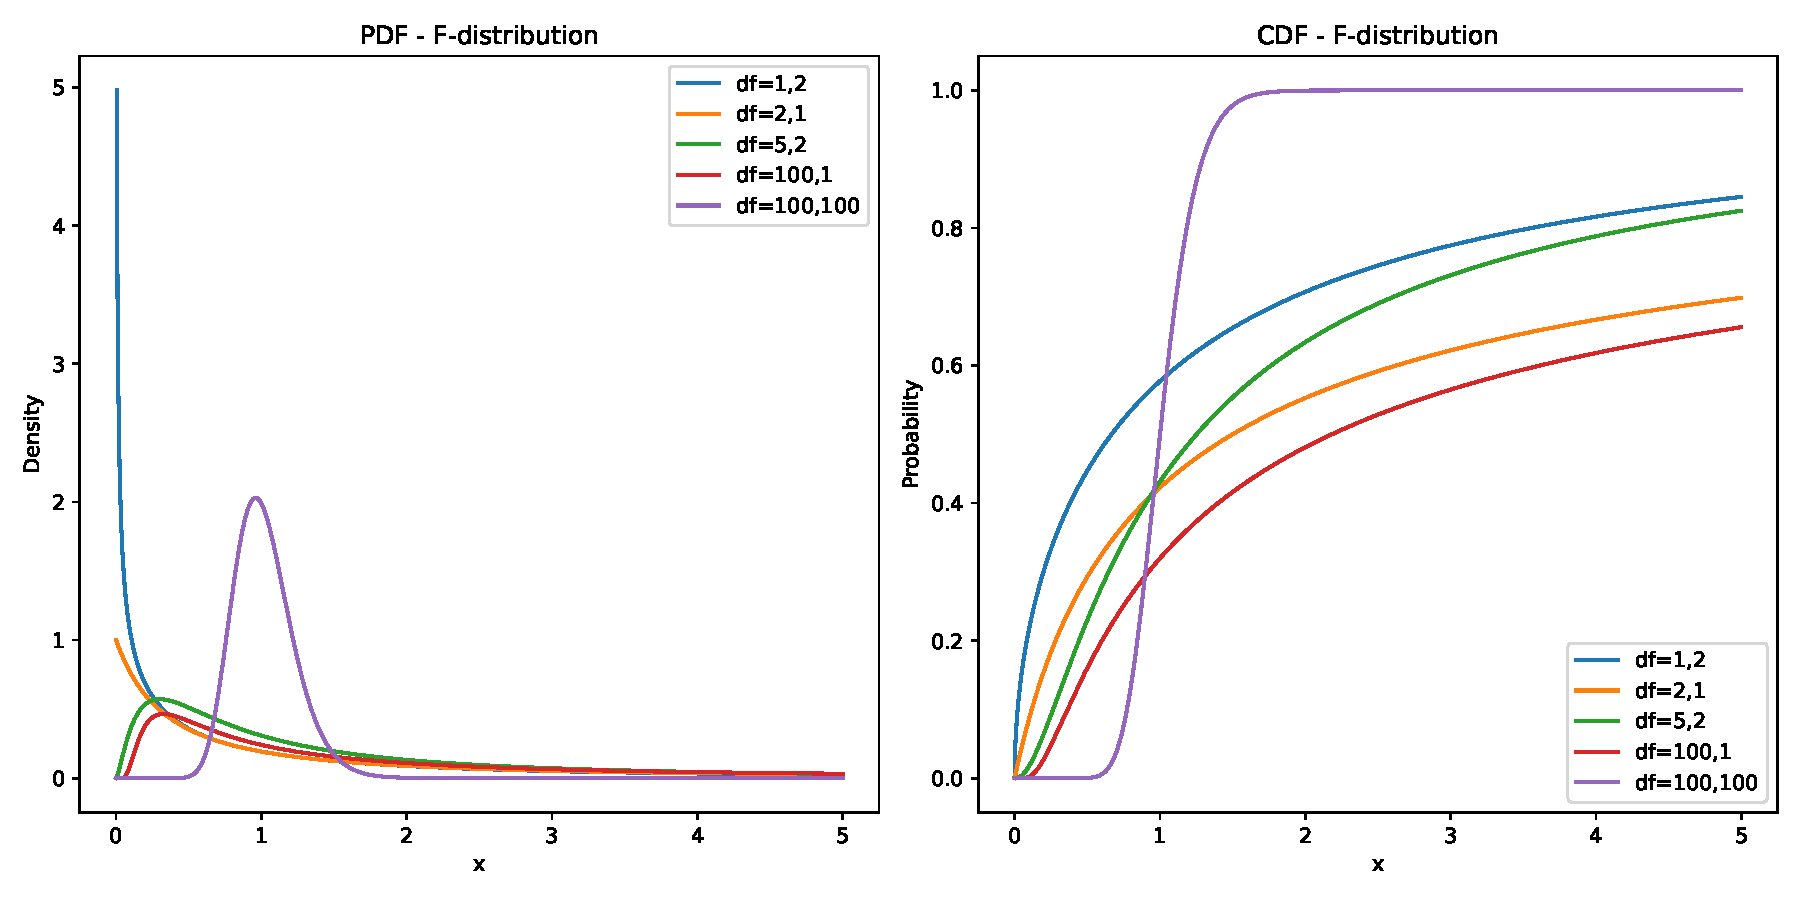
\includegraphics[width=0.8\textwidth]{imgs/F_distribution_plots.pdf}
        \caption{F分布}
        \label{fig:F}
    \end{center}
\end{figure}

使用pdf可以让图表保持为矢量图,不会失真,引入pdf的方式同引入图片的方式一样:表\ref{imgs}

Using pdf can keep the chart as a vector graph, without distortion, the way to introduce pdf is the same as the way to introduce pictures: Listing \ref{imgs}

\subsection{关于页眉页脚 About Header and Footer}

页眉页脚使用 \verb|fancyhdr| 宏包来实现

Header and footer are implemented using the \verb|fancyhdr| package

\begin{lstlisting}[
    style       =   TeX,
    caption     =   {\bf 关于页眉页脚 About Header and Footer},
    label       =   {header}
]
\fancyhf{}
\fancyhead[L]{
    \begin{minipage}[c]{0.2\textwidth}
        \includegraphics[height=11mm]{imgs/logo1.jpg}           %用于设置页眉左侧的图片   Used to set the picture on the left side of the header
    \end{minipage}
}
\fancyhead[C]{实验报告-Experiment report}                        %用于设置页眉中间的文字   Used to set the text in the middle of the header
\fancyfoot[C]{\thepage}
% 设置页眉水平居中
\setlength{\headwidth}{\textwidth}
\fancyhfoffset[L]{\dimexpr0.5\textwidth-0.5\textwidth\relax}
\end{lstlisting}

\subsection{关于封面 About Cover}

我设计了两种封面,一种是用于单人报告的封面,另一种是用于多人报告的封面,文档中展示了两种,可以根据需要选择

I designed two covers, one is for single-person reports, and the other is for multi-person reports. The document shows two types, you can choose according to your needs.

\begin{lstlisting}[
    style       =   TeX,
    caption     =   {\bf 关于封面 About Cover},
    label       =   {cover}
]
\begin{document}
% 切换到单人模式 Switch to single mode
\singlecover

% 切换到多人模式 Switch to multiple mode
\groupcover
\end{document}
\end{lstlisting}

使用时修改前文中的姓名学号等信息,并且选择单人或多人模式,\verb|\singlecover| 是单人模式,\verb|\groupcover| 是多人模式

When using, modify the information such as name and student ID in the previous text, and choose single or multiple mode. \verb|\singlecover| is single mode, and \verb|\groupcover| is multiple mode

\subsection{关于宏包 About Package}

使用了如下宏包:

The following packages are used:

\begin{lstlisting}[
    style       =   TeX,
    caption     =   {\bf 关于Package About Package},
    label       =   {package}
]
\usepackage{geometry} % 用于设置页面布局
\usepackage{authblk}  % 用于处理作者信息
\usepackage{caption}  % 用于生成标题
\usepackage{booktabs} % 用于生成漂亮的表格
\usepackage{hyperref} % 用于添加超链接
\usepackage{cite}     % 用于管理参考文献引用
\usepackage[UTF8]{ctex}% 用于处理中文
\usepackage{graphicx} % 用于插入图片
\usepackage{listings} % 用于插入代码
\usepackage{xcolor}   % 用于设置颜色
\usepackage{abstract} % 用于设置摘要
\usepackage{sectsty}  % 用于设置章节标题
\usepackage{fancyhdr} %用于装饰页脚页眉
\usepackage{multicol} %用于实现多栏排版
\usepackage{amsmath}  %用于数学公式
\usepackage{siunitx}  %用于插入单位
\usepackage{tikz}     %用于绘图
\usepackage{subcaption}%用于插入子图
\end{lstlisting}

\section{个性化 Personalization}

好的排版是满足个性的,这里提供了一些个性化的设置,可以根据自己的需求进行调整

Good typesetting meets individual needs. Here are some personalized settings that can be adjusted according to your needs.

\subsection{字体 Font}

ctex宏包的默认字体是宋体,可以通过设置字体来实现个性化。我自己设置了代码的字体为Consolas,可以根据自己的需求进行调整

The default font of the ctex package is Songti, and personalization can be achieved by setting the font. I set the font of the code to Consolas, which can be adjusted according to your needs.

\vspace{0.5cm}

如果想要更换字体,可以使用 \verb|fontspec| 宏包,例如:

If you want to change the font, you can use the \verb|fontspec| package, for example:

\begin{lstlisting}[
    style       =   TeX,
    caption     =   {\bf 字体设置 Font Setting},
    label       =   {font}
]
\usepackage{fontspec}

\setmainfont{Times New Roman}
\setmonofont{Consolas}
\end{lstlisting}


\subsection{颜色 Color}

颜色可以使用 \verb|xcolor| 宏包来设置,例如:

Colors can be set using the \verb|xcolor| package, for example:

\begin{lstlisting}[
    style       =   TeX,
    caption     =   {\bf 颜色设置 Color Setting},
    label       =   {color}
]
\usepackage{xcolor}

\definecolor{mycolor}{RGB}{255, 110, 0}
\end{lstlisting}

\definecolor{mycolor}{RGB}{255, 110, 0}
比如你想改变一段文字中某些字的颜色,可以使用 \verb|\textcolor{mycolor}{text}|,例如:\textcolor{mycolor}{text}

For example, if you want to change the color of some words in a paragraph, you can use \verb|\textcolor{mycolor}{text}|, for example: \textcolor{mycolor}{text}

\begin{lstlisting}[
    style       =   TeX,
    caption     =   {\bf 颜色使用 Color Using},
    label       =   {coloruse}
]
\textcolor{mycolor}{This is a red text}
\end{lstlisting}

只要你想的话,甚至可以让一段话变成彩虹色:\textcolor{blue}{G}\textcolor{red}{o}\textcolor{yellow}{o}\textcolor{blue}{g}\textcolor{green}{l}\textcolor{red}{e}

If you want, you can even make a paragraph rainbow-colored: \textcolor{blue}{G}\textcolor{red}{o}\textcolor{yellow}{o}\textcolor{blue}{g}\textcolor{green}{l}\textcolor{red}{e}


\begin{lstlisting}[
    style       =   TeX,
    caption     =   {\bf 彩虹 Rainbow Color},
    label       =   {rainbow}
]
\textcolor{blue}{G}\textcolor{red}{o}\textcolor{yellow}{o}\textcolor{blue}{g}\textcolor{green}{l}\textcolor{red}{e}
\end{lstlisting}

\subsection{代码高亮 Code Highlighting}

使用 \verb|listings| 宏包,可以实现代码的高亮显示

Useing the \verb|listings| package, which can highlight code

\subsubsection{已知代码的代码高亮 Code Highlighting for Known Code}

比如Python代码:

For example, Python code:

\begin{lstlisting}[
    style       =   TeX,
    caption     =   {\bf Python代码高亮 Python Code Highlighting},
    label       =   {pythonh}
]
\lstdefinestyle{Python}{
    language        =   Python, % 语言选Python
    frame=single,
    frameround=tttt, % 这个参数设置圆角
    basicstyle      =   \zihao{-5}\ttfamily,
    numberstyle     =   \zihao{-5}\ttfamily,
    keywordstyle    =   \color{blue},
    keywordstyle    =   [2] \color{teal},
    stringstyle     =   \color{magenta},
    commentstyle    =   \color{red}\ttfamily,
    breaklines      =   true,   % 自动换行,建议不要写太长的行
    columns         =   fixed,  % 如果不加这一句,字间距就不固定,很丑,必须加
    basewidth       =   0.5em,
}
\end{lstlisting}

这是在 sty 文件中定义的Python代码高亮样式,然后在代码块中使用 \verb|\lstset{style=Python}| 来应用这个样式,在这里可以调整字体大小、颜色、关键词颜色等

This is the Python code highlighting style defined in the sty file, and then use\\ \verb|\lstset{style=Python}| in the code block to apply this style. Here you can adjust the font size, color, keyword color, etc.

\subsubsection{未知代码的代码高亮 Code Highlighting for Unknown Code}

有些时候我们使用的代码在Latex中并没有定义,这个时候可以先定义一种语言,然后定义一种这种语言的代码高亮样式,例如:

Sometimes the code we use is not defined in Latex. At this time, you can first define a language, and then define a code highlighting style for this language, for example:

\vspace{0.5cm}

比如在我的实验中,我使用了ARM汇编代码,这种代码在Latex中没有定义,所以我先定义了一种ARM汇编语言,然后定义了一种这种语言的代码高亮样式,如下:

For example, in my experiment, I used ARM assembly code, which is not defined in Latex, so I first defined an ARM assembly language, and then defined a code highlighting style for this language, as follows:


\begin{lstlisting}[
    style       =   TeX,
    caption     =   {\bf 未知代码的代码高亮 Code Highlighting for Unknown Code},
    label       =   {unknownh}
]
\lstdefinelanguage{ARMASM}
{
  sensitive=false,
  % base letter (case insensitive)
  morecomment=[l]{//}, % l-line comment
  morecomment=[s]{/*}{*/}, % s-multiline comment
  morestring=[b]", % define strings
  morestring=[b]', % define strings
  morekeywords={
    SVC_Handler, TST, MRSEQ, MRSNE, LDR,
    SUB, AND, CPSID, STRB, MOVS,
    BX, MSR, STR, CPSIE, B
  },
  % list of operators
  morekeywords={[2]
    LR, R1, MSP, PSP, R0,
    SVC_Handler_Main
  },
  % list of other non-standard identifiers
  %stringstyle=\color{cppstring},
  %identifierstyle=\color{blue},
  keywordstyle=\color{blue}\bfseries,
  keywordstyle={[2]\color{green!60!black}\bfseries},
  commentstyle=\color{gray}\textit,
  stringstyle=\color{red},
  % identifierstyle=\color{red},
  % keywordstyle=\color{blue}\bfseries,
  % keywordstyle={[2]\color{green!60!black}\bfseries},
  % commentstyle=\color{gray}\textit,
  % stringstyle=\color{red}
}

\lstdefinestyle{UVisionARMASM}{
    language        =   ARMASM,
    frame=single,
    frameround=tttt, % 这个参数设置圆角
    basicstyle      =   \zihao{-5}\ttfamily,
    numberstyle     =   \zihao{-5}\ttfamily,
    keywordstyle    =   \color{blue}\bfseries,
    keywordstyle    =   [2] \color{green!60!black}\bfseries,  % 设置不同的关键字颜色
    stringstyle     =   \color{red},
    commentstyle    =   \color{gray}\textit,
    breaklines      =   true,
    columns         =   fixed,
    basewidth       =   0.5em,
}
\end{lstlisting}

这是在 sty 文件中定义的ARM汇编代码高亮样式,然后在代码块中使用\\ \verb|\lstset{style=UVisionARMASM}| 来应用这个样式,下面是一个例子:

This is the ARM assembly code highlighting style defined in the sty file, and then use\\ \verb|\lstset{style=UVisionARMASM}| in the code block to apply this style. Here is an example:

\lstinputlisting[
    style       =   UVisionARMASM,
    caption     =   {\bf SVC\_Handler},
    label       =   {svc}
]{codes/svc.s}

\subsection{代码框个性化 Code Box Personalization}

前面代码高亮的定义中,同时也定义了代码框的样式,可以根据自己的需求进行调整,比如:

In the definition of code highlighting above, the style of the code box is also defined, which can be adjusted according to your needs, for example:

\clearpage

\begin{lstlisting}[
    style       =   TeX,
    caption     =   {\bf Python代码高亮 Python Code Highlighting},
    label       =   {pythonh}
]
\lstdefinestyle{Python}{
    language        =   Python, % 语言选Python
    frame=single,
    frameround=tttt,                                % 这个参数设置圆角,t表示圆角,r表示直角 This parameter sets the rounded corners, t means rounded corners, r means right angle
    %frame=shadowbox,                               % 定义是否有阴影 Define whether there is a shadow
    %rulesepcolor=\color{red!20!green!20!blue!20},  % 定义阴影颜色 Define shadow color
    basicstyle      =   \zihao{-5}\ttfamily,
    numberstyle     =   \zihao{-5}\ttfamily,
    keywordstyle    =   \color{blue},
    keywordstyle    =   [2] \color{teal},
    stringstyle     =   \color{magenta},
    commentstyle    =   \color{red}\ttfamily,
    breaklines      =   true,   % 自动换行,建议不要写太长的行
    columns         =   fixed,  % 如果不加这一句,字间距就不固定,很丑,必须加
    basewidth       =   0.5em,
}
\end{lstlisting}

下面是一些例子:

Here are some examples:

\begin{lstlisting}[
    style       =   PythonR,
    caption     =   {\bf 直角代码框 Right Angle Code Box},
    label       =   {pythonh}
]
'''
frameround=rrrr, % 这个参数设置直角
'''

print("Hello World!")
\end{lstlisting}

\begin{lstlisting}[
    style       =   PythonS,
    caption     =   {\bf 阴影代码框 Shadow Code Box},
    label       =   {pythonh}
]
'''
frameround=rrrr, % 这个参数设置直角
frame=shadowbox,                               % 定义是否有阴影 Define whether there is a shadow
rulesepcolor=\color{red!20!green!20!blue!20},  % 定义阴影颜色 Define shadow color
'''

print("Hello World!")
\end{lstlisting}

\clearpage

\begin{lstlisting}[
    style       =   PythonFuck,
    caption     =   {\bf 乱写代码框 Random Code Box},
    label       =   {pythonh}
]
'''
frameround=trtr, % 这个参数设置直角
frame=shadowbox,                               % 定义是否有阴影 Define whether there is a shadow
rulesepcolor=\color{red!20!green!20!blue!20},  % 定义阴影颜色 Define shadow color
'''

print("Hello World!")
\end{lstlisting}

谨慎使用圆角和阴影,因为阴影没有圆角。如果你想要圆角阴影,请使用tcolorbox宏包,具体的使用请查看:\href{https://wenda.latexstudio.net/data/ueditor/php/upload/file/20190817/1566001633576064.pdf}{这篇文章}

Be sparing with rounded corners and shadows, as shadows do not have rounded corners. If you want rounded shadows, please use the tcolorbox macro package, please see: \href{https://wenda.latexstudio.net/data/ueditor/php/upload/file/20190817/1566001633576064.pdf}{this article}

\subsection{修改超链接颜色 Change Link Color}

\begin{lstlisting}[
    style       =   TeX,
    caption     =   {\bf 修改超链接颜色 Change Link Color},
    label       =   {linkcolor}
]
% 设置超链接颜色
\hypersetup{
    colorlinks=true,
    linkcolor=blue, % 超链接的颜色
    urlcolor=red,   % URL 的颜色
    citecolor=green % 引用的颜色
}
\end{lstlisting}

我希望目录保持原来的黑色,所以我在目录外面包裹了颜色修改,这样目录就不会变成蓝色了

I want the directory to remain black, so I wrapped the color change outside the directory, so the directory will not turn blue

\begin{lstlisting}[
    style       =   TeX,
    caption     =   {\bf 修改目录链接颜色 Change Link Color in Table of Contents},
    label       =   {toclinkcolor}
]
\hypersetup{linkcolor=black}
\tableofcontents
\hypersetup{linkcolor=blue}
\end{lstlisting}

\section{总结 Summary}

这篇文章简单的介绍了一些Latex的使用方法以及这个实验报告模板的使用,希望能够在你写报告的时候能有所帮助!如果你有建议和修改请联系 \href{2861126078@qq.com}{2861126078@qq.com}

This article briefly introduces some of the ways to use Latex and the use of this lab report template, I hope it can be helpful when you write your report! If you have suggestions or modifications, please contact \href{2861126078@qq.com}{2861126078@qq.com}


\section*{附录 Appendix}
\addcontentsline{toc}{section}{附录 Appendix}

这里是附录,一般会放上一些完整代码和实验结果图片还有参考文献

Here is the appendix, which generally contains some complete code, experimental result pictures, and references


\begin{thebibliography}{9}
    \bibitem{1} Gao P H. SDU \LaTeX \ Template[J]. 2024
\end{thebibliography}



\end{document}